%%% mode: latex; mode:flyspell
%%%%%%%%%%%%%%%%%%%%%%%%%%%%%%%%%%%%%%%%%%%%%%%%%%%%%%%%%%%%%%%%%%%%%%%%%%%%% 
\section{Track momentum corrections}

The mean value of the reconstructed track momentum extrapolated to the tracker entrance is
slightly lower than the true MC momentum of the corresponding MC particle at the tracker entrance.
The offset is on the order of 30 keV/c and depends on the ambiguity resolver used in the track fit.
We correct the reconstructed momentum of PAR tracks by 34 keV/c and DAR tracks by 30 keV/c.

{\blue PAR and DAR are introduced in the next section but should be defined here}

\begin{figure}[h]
\hspace{-0.6in}
\begin{tikzpicture}
  \node[anchor=south west,inner sep=0] at (0,0.) {
    % \node[shift={(0 cm,0.cm)},inner sep=0,rotate={90}] at (0,0) {}
    % \makebox[\textwidth][c] {
      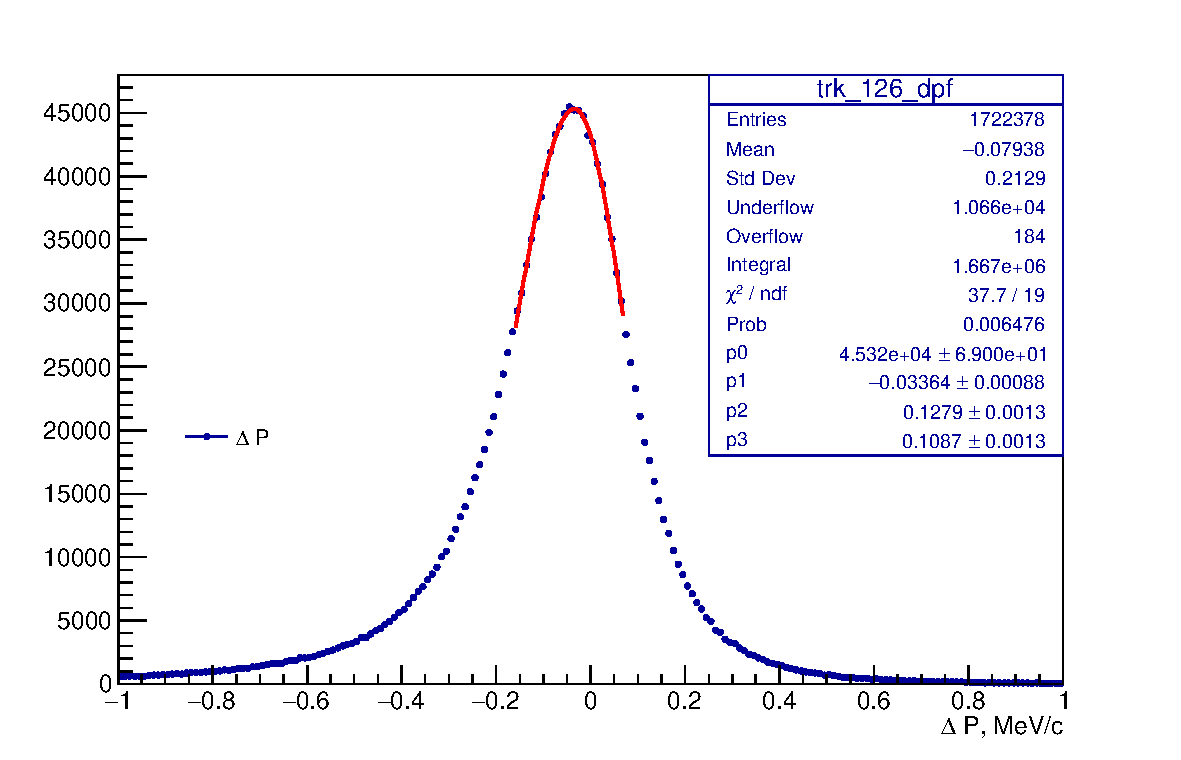
\includegraphics[width=0.6\textwidth]{figures/pdf/figure_00112_fele2s51b1_track_comp_ffff_1070_nocorr_trk_126_dpf}
    %}
  };
  \node[anchor=south west,inner sep=0] at (10,0.) {
    % \node[shift={(0 cm,0.cm)},inner sep=0,rotate={90}] at (0,0) {}
    % \makebox[\textwidth][c] {
      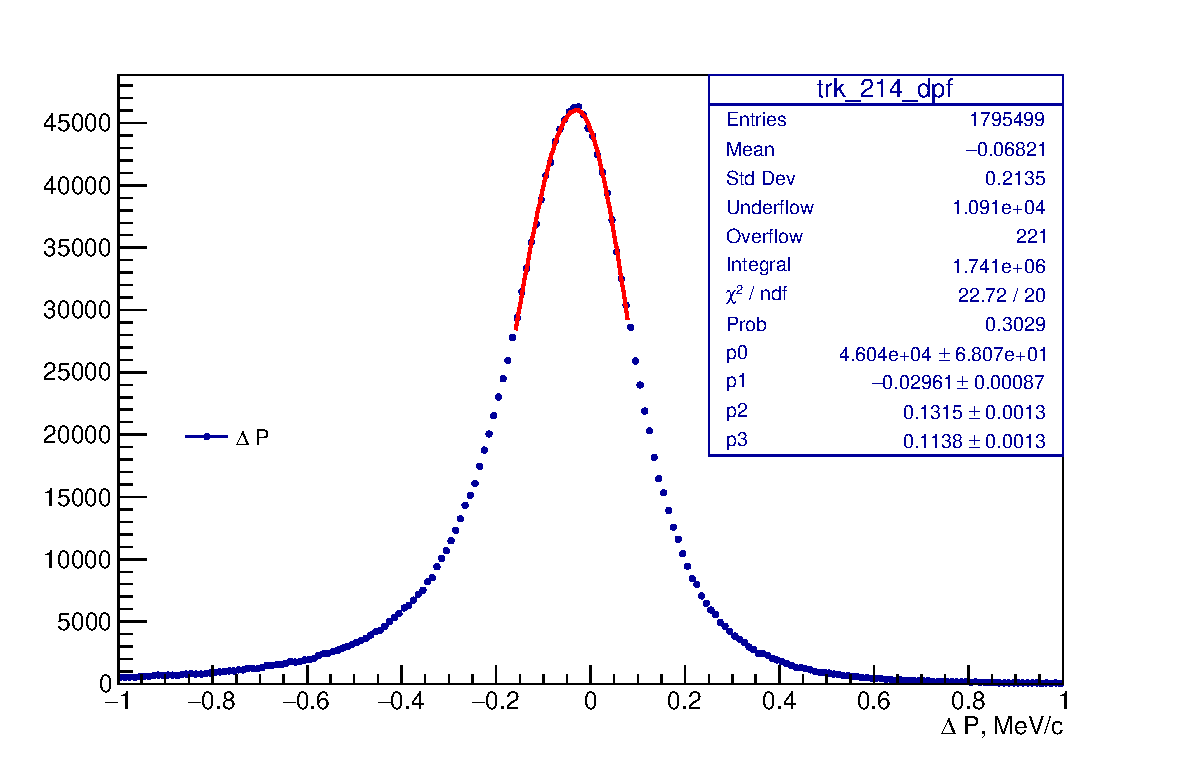
\includegraphics[width=0.6\textwidth]{figures/pdf/figure_00113_fele2s51b1_track_comp_ffff_1070_nocorr_trk_214_dpf}
    %}
  };
  % \node [text width=6cm, scale=0.8] at (4.5,6.4) {mu2e-18894 by Kevin Lynch and Jim Popp};
\end{tikzpicture}

\caption{
  \label{fig:sindrum_ii_fig_08_fit} 
  $\Delta P = P_{\rm rec} - P_{\rm MC}$ distributions at the tracker front for PAR (left) and DAR (right) tracks.
  The distributions are fit with an asymmetric ($\sigma_{left} \ne \sigma_{right}$) Gaussian function. 
  The peak positions are used to correct the reconstructed momentum of tracks returned by the respective fits.
}
\end{figure}


%%% Local Variables:
%%% TeX-master: "mu2e-36575"
%%% End:
